\section{Declaring Correspondences between two Graphs}

First, we will create a TGG project, which is the correspondence component
in the triple graph structure, and declare the \emph{correspondency types}
between classes from \texttt{LearningBoxLanguage} and
\texttt{DictionaryLanguage}.
As hinted above, a \emph{correspondency type} can be considered as a
traceability link which interrelates the elements from source and target
components in a bidirectional transformation.

In EA, add a new package and enter
\texttt{Learning\-Box\-To\-Dictionary\-Integration} as its name. Create a
diagram for the new package and select \texttt{TGGSchema} as diagram type
(Fig.~\ref{fig:tgg_diagram_type}). This way, we determine our new package as a TGG Project. After choosing \texttt{TGGSchema} as diagram type, a new dialog pops up
which asks you for the source and target for your TGG project. Choose
\texttt{Learning\-Box\-Language} as source and \texttt{Dictionary\-Language} as
target project and click \texttt{OK} (Fig.~\ref{fig:select_source_target}).

\begin{figure}[htbp]
\begin{center}
  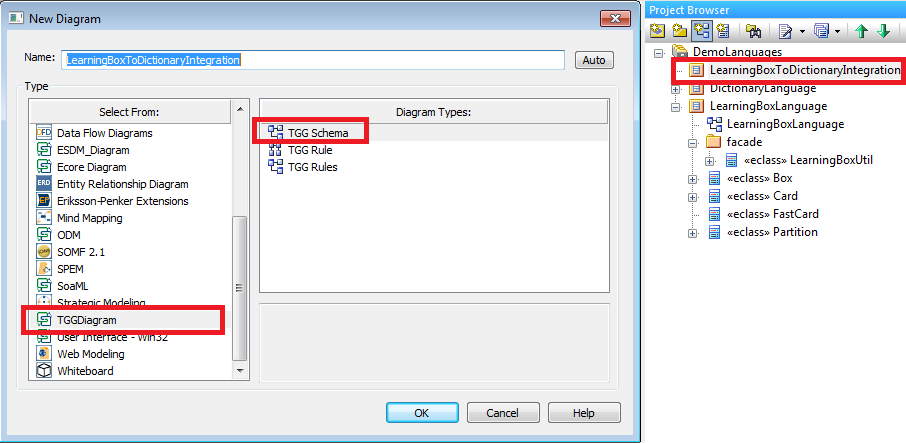
\includegraphics[width=\textwidth]{pics/tggBilder/tgg1}
  \caption{Choosing \texttt{TGGSchema} as your diagram type}  
  \label{fig:tgg_diagram_type}
\end{center}
\end{figure}

\begin{figure}[htbp]
\begin{center}
  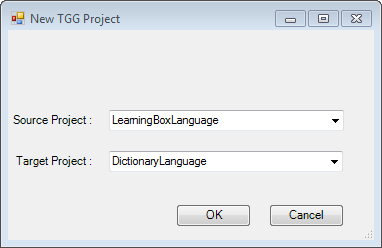
\includegraphics[width=0.4\textwidth]{pics/tggBilder/tgg2}
  \caption{Selecting a source and target project for a TGG project}  
  \label{fig:select_source_target}
\end{center}
\end{figure}

The structure of your TGG project should resemble
Fig.~\ref{fig:new_tgg_project}. Please note that a subpackage \texttt{Rules} and an underlying diagram with the same name are
also generated.

\begin{figure}[htbp]
\begin{center}
  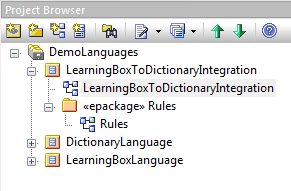
\includegraphics[width=0.4\textwidth]{pics/tggBilder/tgg3}
  \caption{The new TGG Project with its generated subpackage \texttt{Rules}}  
  \label{fig:new_tgg_project}
\end{center}
\end{figure}

Now, it's time to insert classes from our source and target projects
into our TGG project and declare our first correspondency between them. The
classes \texttt{Box} and \texttt{Dictionary}, both being at the top of the composite hierarchy in their own languages,
should be related to each other for our bidirectional transformation. Drag
\& drop the class \texttt{Box} in \texttt{Learning\-Box\-Language} from the project 
browser to the newly created diagram
\texttt{Learning\-Box\-To\-Dictionary\-Integration}. Please assure that the
class is pasted \texttt{as simple link} into the diagram as depicted in
Fig.~\ref{fig:drag_drop_box}. 

\begin{figure}[htbp]
\begin{center}
  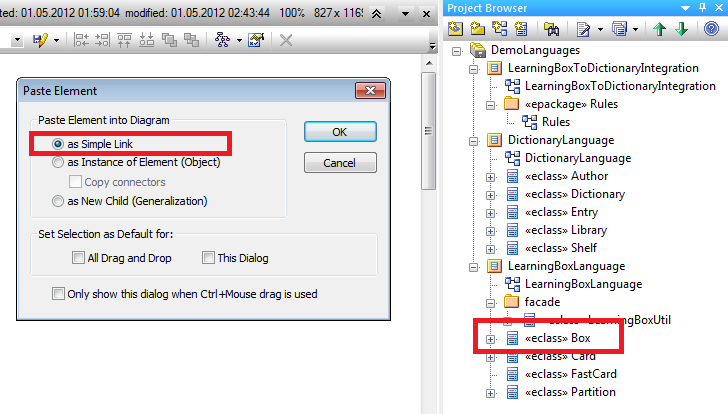
\includegraphics[width=0.6\textwidth]{pics/tggBilder/tgg4}
  \caption{Drag \& Drop \texttt{Box} as simple link} 
  \label{fig:drag_drop_box}
\end{center}
\end{figure}

If the dialog in Fig.~\ref{fig:drag_drop_box} doesn't show up
and the class is somehow not being pasted as simple link, hold down
\texttt{Ctrl} and drag \& drop again.

In the same way, drag \& drop the class \texttt{Dictionary} from
\texttt{Dictionary\-Language} to the diagram. Now, having one class each from
source and target project, we can create a correspondence type between them.
Pull a quick link from \texttt{Box} to \texttt{Dictionary} and in the opened menu select \texttt{Create TGG Correspondence Type} as depicted in Fig.~\ref{fig:create_correspondence}.

\begin{figure}[htbp]
\begin{center}
  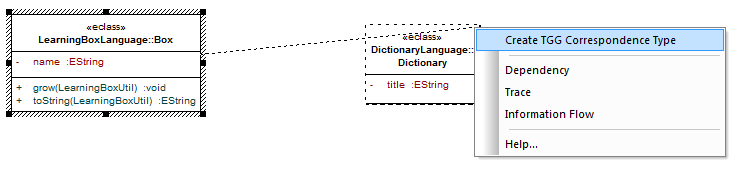
\includegraphics[width=\textwidth]{pics/tggBilder/tgg5}
  \caption{creating a TGG Correspondence Type} 
  \label{fig:create_correspondence}
\end{center}
\end{figure}

A hexagon-shaped \texttt{CorrespondenceType} with the name
\texttt{BoxToDictionary} will be created. Also the connectors to the source and
target elements are generated, so that your diagram resembles
Fig.~\ref{fig:first_correspondence}.

\begin{figure}[htbp]
\begin{center}
  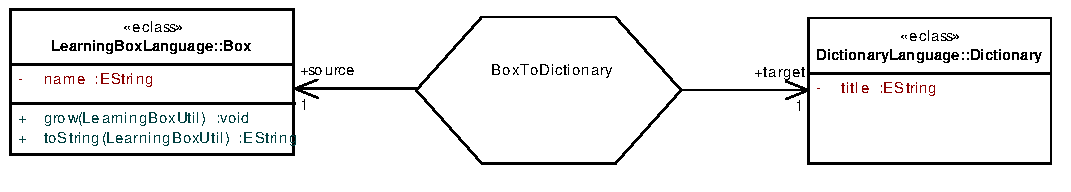
\includegraphics[width=\textwidth]{pics/tggBilder/tgg6}
  \caption{a TGG Correspondence Type between \texttt{Box} and
  \texttt{Dictionary}}
  \label{fig:first_correspondence}
\end{center}
\end{figure}

The last thing to do in this chapter is to declare a further correspondence type
between \texttt{Card} and \texttt{Entry}. Drag \& drop these classes as simple
link to your diagram end create a correspondence type using the same concepts.
The complete TGG Schema diagram is depicted in
Fig.~\ref{fig:complete_tgg_schema}.

\begin{figure}[htbp]
\begin{center}
  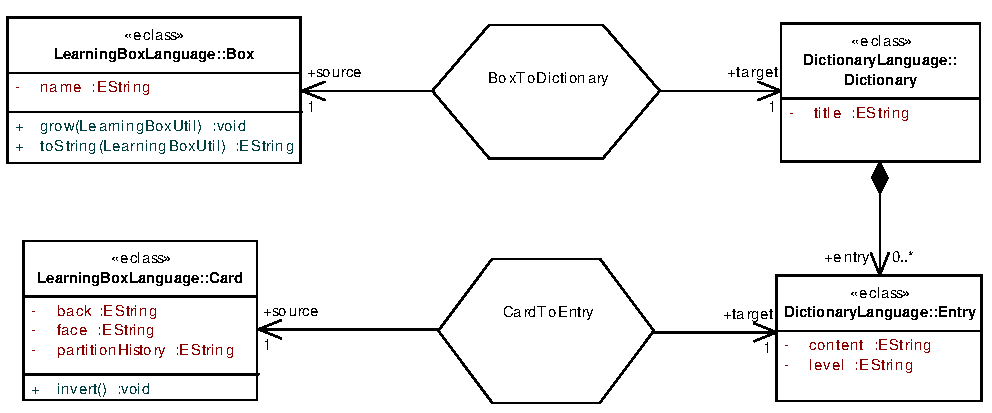
\includegraphics[width=\textwidth]{pics/tggBilder/tgg7}
  \caption{Complete TGG Schema Diagram}
  \label{fig:complete_tgg_schema}
\end{center}
\end{figure}
